\chapter{Graph Games}
This section gives an alternative definition of a combinatorial game.
This definition allows us to study general combinatorial games.
\begin{definition}
  A \emph{directed graph} $G$ is a pair $(V, N)$ such that $F$ is a non-empty
  set and $F : V \to 2^V$.\footnote{%
    We are going to have a more in-depth
    discussion of graphs in \Cref{part:graph-theory}.
  }

  We say that a game on $G$ is the impartial game where elements of $V$ are
  positions and each player can move from $x \in V$ to any $y \in N(x)$.
  (Elements of $N(x)$ are called followers of $x$.)
\end{definition}

\begin{remark}
  It is also easy to see that any impartial game can be transformed into a graph
  $G$ such that the game on $G$ and the impartial game are equivalent.
\end{remark}

For example, the take-away game from \Cref{chapter:combinatorial-games}
can be considered as a graph on a graph $G = (\N_0, N)$,
where $N(0) = \emptyset$, $N(1) = \set{0}$, $N(2) = \set{0, 1}$, and
$N(n + 3) = \set{n, n + 1, n + 2}$ for any $n \in \N_0$.

The key ingredient for the analysis of games based on graphs was proposed
by Sprague and Grundy. They proposed to consider the following function:
\begin{definition}
  Let $G = (V, N)$ be a directed graph. A function $g : V \to \N$ is a
  \emph{Sprague--Grundy function} for $G$ iff
  $g(x) = \mex\set[y \in N(x)]{g(y)}$, where
  $\mex S = \min \set[n \notin S]{n \in \N_0}$.
\end{definition}


Consider the following graph (arrows depict possible moves).
\begin{center}
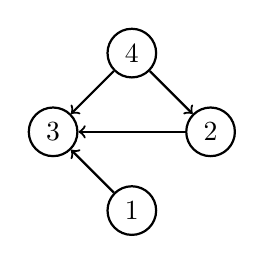
\begin{tikzpicture}[thick]
  \node[circle, draw, minimum size=6pt] (v1) at (0,0) {$1$};
  \node[circle, draw, minimum size=6pt] (v2) at (1,1) {$2$};
  \node[circle, draw, minimum size=6pt] (v3) at (-1,1) {$3$};
  \node[circle, draw, minimum size=6pt] (v4) at (0,2) {$4$};


  \draw[->] (v2) -- (v3);
  \draw[->] (v1) -- (v3);
  \draw[->] (v4) -- (v3);
  \draw[->] (v4) -- (v2);
\end{tikzpicture}
\end{center}
Let us assume that $g$ is a Sprague--Grundy function for this graph.
Note that $3$ is a terminal position so $g(3) = \mex \emptyset = 0$.
Since from $1$ and $2$ there are only moves to $3$, it is clear that
$g(1) = g(2) = \mex \set{0} = 1$. Finally, $g(4) = \mex \set{0, 1} = 2$.

Note that the Sprague--Grundy function is recursively defined so it may
not exist or not to be unique if graph violets the ending condition.
For example, the graph depicted on \Cref{figure:sprague-grundy-not-exists}
does not have a Sprague--Grundy function.
Indeed, assume that such a function $g$ exists. Consider two following cases.
\begin{itemize}
    \item Firs case is when $g(3) = 0$. Note that $g(2) = \mex \set{0} = 1$.
        Hence, $g(1) = \mex \set{1} = 0$ which contradicts to the assumption
        that $g(3) = 0$ since $g(3) = \mex \set{g(0)} = 1$.
    \item Firs case is when $g(3) \neq 0$. Note that $g(2) = \mex \set{g(3)} = 0$.
        Therefore $g(1) = \mex \set{0} = 1$ and $g(3) = \mex \set{1} = 0$ which
        is a contradiction.
\end{itemize}

Note that the graph depicted on \Cref{figure:sprague-grundy-not-unique} has
several Sprague--Grundy functions. We may consider functions $g_1$ and $g_2$
such that $g_1(1) = g_1(3) = g_2(2) = g_2(4) = 0$ and
$g_2(1) = g_2(3) = g_1(2) = g_1(4) = 1$. It is clear that they are
Sprague--Grundy functions for the graph from
\Cref{figure:sprague-grundy-not-unique}.

\begin{figure}
    \centering
    \subfloat[A graph without a Sprague--Grundy function
              \label{figure:sprague-grundy-not-exists}]{
      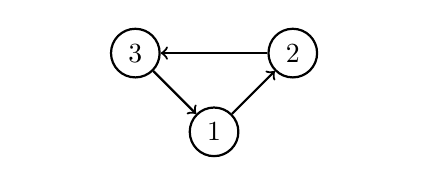
\begin{tikzpicture}[thick]
        \node[circle, draw, minimum size=6pt] (v1) at (0,0) {$1$};
        \node[circle, draw, minimum size=6pt] (v2) at (1,1) {$2$};
        \node[circle, draw, minimum size=6pt] (v3) at (-1,1) {$3$};
        \node[] (dummy) at (2.25,1) {};
        \node[] (dummy) at (-2.25,1) {};

        \draw[->] (v1) -- (v2);
        \draw[->] (v2) -- (v3);
        \draw[->] (v3) -- (v1);
      \end{tikzpicture}
    }
    \qquad
    \subfloat[A graph with several Sprague--Grundy functions
              \label{figure:sprague-grundy-not-unique}] {
      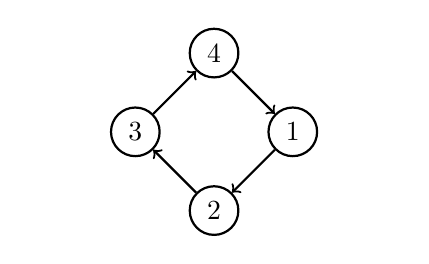
\begin{tikzpicture}[thick]
        \node[circle, draw, minimum size=6pt] (v1) at (1,1) {$1$};
        \node[circle, draw, minimum size=6pt] (v2) at (0,0) {$2$};
        \node[circle, draw, minimum size=6pt] (v3) at (-1,1) {$3$};
        \node[circle, draw, minimum size=6pt] (v4) at (0,2) {$4$};
        \node[] (dummy) at (2.25,1) {};
        \node[] (dummy) at (-2.25,1) {};


        \draw[->] (v1) -- (v2);
        \draw[->] (v2) -- (v3);
        \draw[->] (v3) -- (v4);
        \draw[->] (v4) -- (v1);
      \end{tikzpicture}
    }
    \caption{Graphs where Sprague--Grundy function is either not unique or does
      not exist.}
    \vskip 10pt
\end{figure}

Unfortunately, even if there are no cycles, a graph my not have a
Sprague--Grundy function or have several Sprague--Grundy functions. Indeed,
consider the graph $G = (\Z, N)$ such that $N(x) = \set{x - 1}$. It is clear
that the functions $g_1$ and $g_2$ such that
\begin{gather*}
    g_1(x) =
    \begin{cases}
        0 & \text{if } x \text{ is even} \\
        1 & \text{if } x \text{ is odd}
    \end{cases} \\
    \text{and} \\
    g_2(x) =
    \begin{cases}
        0 & \text{if } x \text{ is even} \\
        1 & \text{if } x \text{ is odd}
    \end{cases}
\end{gather*}
are Sprague--Grundy functions for $G$.

\begin{exercise}
    Let $G = (\N \cup \set{\infty}, N)$ such that 
    $N(x) = \set[y < x]{y \in \N_0}$, and $N(\infty) = \N$.
    Show that $G$ does not have a Sprague--Grundy function.
\end{exercise}

However, all the combinatorial games we are going to consider
the Sprague--Grundy function exists and is unique.
\begin{theorem}
\label{theorem:ending-condition-sg-function}
  Let $G = (V, N)$ be a graph such that $N(v)$ is finite and $G$ satisfies the
  ending condition. Then Sprague--Grundy function for $G$ exists and it is
  unique.
\end{theorem}

Before we prove this theorem, let us illustrate by proving that the
Sprague--Grundy function for \Cref{game:take-away-21-3-2-1} is unique.
Assume that a Sprague--Grundy function $g$ for \Cref{game:take-away-21-3-2-1}
exists. We are going to show that it is unique.
Note that if $x$ is a terminal position, then $g(x) = 0$. Hence, $g(0) = 0$.
There is only one move from $1$ so $g(1) = \mex \set{0} = 1$. Similarly
there are two moves from $2$: one to $1$ and one to $0$ so
$g(2) = \mex \set{0, 1} = 2$. In the same way $g(3) = \mex \set{0, 1, 2} = 3$
and $g(4) = \mex \set{1, 2, 3} = 0$.
One may notice that there is a pattern and conjecture that
\[
  g(x) =
  \begin{cases}
      0 & \text{if } x \equiv 0 \pmod{4} \\
      1 & \text{if } x \equiv 1 \pmod{4} \\
      2 & \text{if } x \equiv 2 \pmod{4} \\
      3 & \text{if } x \equiv 3 \pmod{4}
  \end{cases}.
\]
We already proved the base case, let us now prove the induction step.
Assume the equality is true for all $y < x$ and consider the following cases.
\begin{itemize}
    \item If $x \equiv 0 \pmod{4}$, then $x - 1 \equiv 3 \pmod{4}$,
        $x - 2 \equiv 2 \pmod{4}$, and $x - 3 \equiv 1 \pmod{4}$.
        Hence, $g(x) = \mex \set{1, 2, 3} = 0$.
    \item If $x \equiv 1 \pmod{4}$, similarly $g(x) = \mex \set{2, 3, 0} = 1$.
    \item If $x \equiv 2 \pmod{4}$, $g(x) = \mex \set{3, 0, 1} = 2$.
    \item If $x \equiv 3 \pmod{4}$, $g(x) = \mex \set{0, 1, 2} = 3$.
\end{itemize}
It is also clear that the constructed function is indeed a Sprague--Grundy
function for \Cref{game:take-away-21-3-2-1}. Therefore we proved that
existence and uniqueness.
\begin{table}
  \centering
  \begin{tabular}{l l l l l l l l l}
      \toprule
      0 & 1 & 2 & 3 & 4 & 5 & 6 & 7 & 8 \\
      \midrule
      0 & 1 & 2 & 3 & 0 & 1 & 2 & 3 & 0 \\
      \bottomrule
  \end{tabular}
  \caption{The Sprague--Grundy function for \Cref{game:take-away-21-3-2-1}}
  \label{table:take-away-21-3-2-1-grundy}
  \vskip 10pt
\end{table}

Note that in this proof we used a procedure very similar to the one we used to
find P- and N-positions.
\begin{template}
  \textbf{Steps necessary to find a Sparague--Grundy function} \\

  Assume we are trying to construct a a Sparague--Grundy function $g$.
  \begin{enumerate}
    \item Set $g(x) = 0$ for all terminal positions $x$.
    \item If $g(x)$ is not defined but $g(y)$ is defined for all $y \in N(x)$,
      then set $g(x) = \mex \set[y \in N(x)]{g(y)}$.
    \item If $g(x)$ is not defined for some $x$, go to Step~2.
  \end{enumerate}
\end{template}

Let $V_0$ be the set of terminal positions, and let $V_i$ be the set of $x$ such
that we define $g(x)$ on the $i$th iteration of the procedure.
The following lemma eseentially says that this procedure defines $g$ everywhere.
\begin{lemma}[K\H{o}nig]
\label{lemma:konig}
  Let $G = (V, N)$ be a graph such that $N(v)$ is finite for all $v \in V$ and
  $G$ satisfies the ending condition.
  Let $V_0$ be the set of terminal positions, and let $V_{n + 1} = 
  \set[N(v) \subseteq V_n]{v \in V}$. Then $V = \bigcup_{n \in \N_0} V_n$.
\end{lemma}

\begin{proof}[Proof of \Cref{theorem:ending-condition-sg-function}]
  Let $V_0$ be the set of terminal positions, and let $V_{n + 1} = 
  \set[N(v) \subseteq V_n]{v \in V}$.
  \Cref{lemma:konig} claims that $V = \bigcup_{n \in \N_0} V_n$.

  For each $n \in \N_0$, we define $g_n : V_n \to \N_0$ such that 
  $
    g_{n + 1}(v) = \mex \set[u \in N(v)]{g_n(u)}
  $
  for $v \in V_{n + 1}$ and $g_0(v) = 0$ for $v \in V_0$. It is easy to see
  that the function $g : V \to \N_0$ such that $g(v) = g_n(v)$ for $v \in V_n$
  is a Sprague--Grundy function for $G$. 

  To finish the proof we need to prove that there are no other Sprague--Grundy
  functions for $G$. Assume that $g'$ is a Sprague--Grundy function for
  $G$; we prove using induction by $n \in \N_0$ that $g(v) = g'(v)$ for 
  $v \in V_n$. The base case for $v = 0$ is clear since $N(v) = \emptyset$ for
  $v \in V_0$. Let us consider the induction step from $n$ to $n + 1$. By the
  induction hypothesis, $g(u) = g'(u)$ for $u \in V_n$. Let us consider some $v
  \in V_{n + 1}$. Note that 
  \[
    g'(v) = \mex \set[u \in N(v)]{g(u)} = \mex \set[u \in N(v)]{g(u)} = g(v).
  \]
  Therefore $g(v) = g'(v)$ for $v \in V_{n + 1}$. As a result, $g(v) = g'(v)$
  for $v \in V$; i.e., $g = g'$.
\end{proof}

One may note that in \Cref{game:take-away-21-3-2-1} P-positions are the positions
where the Sprague--Grundy function is zero. In fact, this is not a coincidence.
\begin{theorem}
\label{theorem:grundy-to-np}
  Let $G = (V, N)$ be a graph such that $N(v)$ is finite for all $v \in V$ and 
  $G$ satisfies the ending condition. Then all the vertices of $G$ can be
  labeled as either P- or N-positions. Moreover, $v \in V$ is a P-position iff
  $g(v) = 0$, where $g$ is the Sprague--Grundy function for $G$.
\end{theorem}


\begin{chapterendexercises}
    \exercise Prove \Cref{theorem:grundy-to-np}.
    \exercise Show that there are only two Sprague--Grundy functions for the
      graph depicted on \Cref{figure:sprague-grundy-not-unique}.
    \exercise Prove that there is unique Sprague--Grundy function for the one pile
        Nim game.
    \exercise Prove that there is unique Sprague--Grundy function for the
        subtraction game where players may subtract $2$ and $3$ chips on their
        turn.
    \exercise
       Prove that there is unique Sprague--Grundy function for the subtraction
       game where players may subtract $1$, $2$, or $5$ chips
       on their turn.
\end{chapterendexercises}
